\documentclass[letterpaper, 10pt, conference]{ieeeconf}  % Comment this line out if you need a4paper

\IEEEoverridecommandlockouts                              % This command is only needed if
                                                          % you want to use the \thanks command

\overrideIEEEmargins                                      % Needed to meet printer requirements.

%In case you encounter the following error:
%Error 1010 The PDF file may be corrupt (unable to open PDF file) OR
%Error 1000 An error occurred while parsing a contents stream. Unable to analyze the PDF file.
%This is a known problem with pdfLaTeX conversion filter. The file cannot be opened with acrobat reader
%Please use one of the alternatives below to circumvent this error by uncommenting one or the other
%\pdfobjcompresslevel=0
%\pdfminorversion=4

% See the \addtolength command later in the file to balance the column lengths
% on the last page of the document

% numbers option provides compact numerical references in the text.
% \usepackage{natbib}
\let\proof\relax
\let\endproof\relax
\usepackage{amsthm}
\usepackage{times}
\usepackage{multicol}
\usepackage[bookmarks=true]{hyperref}
\usepackage{xcolor}
\usepackage{hyperref}
\usepackage{amsmath, amssymb}
\usepackage{amsfonts}
\usepackage{graphicx}
\usepackage{siunitx}
\usepackage{standalone}
\usepackage{booktabs}
\usepackage[ruled,vlined,linesnumbered,noend]{algorithm2e}
\usepackage{mdframed}
\usepackage{fancyvrb,multirow}
\usepackage{soul}
\usepackage{dsfont,mathabx}
\usepackage{array, booktabs}
\usepackage{subfigure}
\usepackage{booktabs}
\usepackage{makecell}
\usepackage{threeparttable}

%%============================
%%============================

\newtheorem{theorem}{Theorem}
\newtheorem{proposition}{Proposition}
\newtheorem{lemma}{Lemma}
\theoremstyle{definition}
\newtheorem{assumption}{Assumption}
\newtheorem{definition}{Definition}
\newtheorem{remark}{Remark}
\newtheorem{example}{Example}
\newtheorem{problem}{Problem}

% GENERAL
\newcommand{\todo}[1]{\textcolor{red}{TODO: #1}}
\newcommand{\improve}[1]{\textcolor{cyan}{#1}}
\newcommand{\note}[1]{\textcolor{blue}{NOTE: #1}}
\newcommand{\question}[1]{\textcolor{orange}{Q: #1}}
\newcommand{\wnote}[1]{\textcolor{teal}{W: #1}}

%%%%%%%%%%%%%%%%%%%%%%%%%%%%%%%%%%%%%%%%%%%%%%%%%%%%%%%
%%%%


\title{\textbf{BodyGuards: Escorting by Multiple Robots in Unknown Environment\\
under Limited Communication}}


\author{Zhuoli Tian, Yanze Bao and Meng Guo$^*$% <-this % stops a space
  \thanks{$^*$This work was supported by the National Natural Science Foundation of China
    (NSFC) under grants U2241214, T2121002. Corresponding author:
    Meng Guo, meng.guo@pku.edu.cn.}% <-this % stops a space
  }


\begin{document}
\maketitle
\thispagestyle{empty}
\pagestyle{empty}


%%========================================


%%========================================
\begin{abstract}
Heterogeneous multi-arm manipulation can combine complementary workspaces,
end-effectors, and sensing capabilities for concurrent task execution in
dynamic workspaces. However, semantic coordination becomes difficult when the
physical scene changes continually while task-relevant updates, external
disturbances, and execution failures occur only at discrete moments. Static or
monolithic semantic coordination can either miss these events or trigger
unnecessary global replanning that interrupts still-valid execution. This work
addresses this problem through role-shared semantic coordination for dynamic
heterogeneous multi-manipulator scenarios. The framework assigns explicit
semantic responsibilities to the affordance, planning, and verification roles
over a shared semantic state that stores the current instruction, the
assignment-aware primitive graph, task-relevant scene facts, and execution
status. An event-driven selective semantic update procedure further identifies
the affected scope caused by a task update, external disturbance, or execution
failure, and revises only that scope while preserving unaffected valid
execution. Simulation baselines, failure analysis, and ablations show that
explicit responsibility separation reduces coordination errors and selective
semantic updates enable faster adaptation in evolving environments; hardware
trials examine the same mechanisms on a heterogeneous multi-arm platform.
\end{abstract}

%%========================================
\section{Introduction}
\label{sec:introduction}

\providecommand{\introchange}[1]{#1}
\providecommand{\structurechange}[1]{#1}
\providecommand{\localexecchange}[1]{#1}

Heterogeneous multi-manipulator systems must maintain a consistent task
interpretation while complementary robots execute concurrently in a changing
workspace. Figure~\ref{fig:scenario} instantiates this problem with a conveyor
and three task-relevant semantic events. Language- and vision-language-based
grounding~\cite{huang2023inner,liang2023code,rana2023sayplan} does not expose
team capability constraints or
responsibility interfaces; independent agents can therefore maintain
incompatible task views. The challenge is to
establish one capability-aware semantic authority across robots and revise only
the semantics invalidated by a new instruction, disturbance, or verified
failure while local controllers remain responsive to continuous scene
evolution. We propose RoSC, a role-shared semantic coordination framework with
an event-driven selective update that follows event detection $\rightarrow$
affected-scope selection $\rightarrow$ semantic-state revision $\rightarrow$
continued dispatch from a consistent frontier. Simulation baselines, failure
analysis, and mechanism ablations test these mechanisms, while hardware trials
check the same update sequence during physical execution.

\begin{figure}[t]
    \centering
    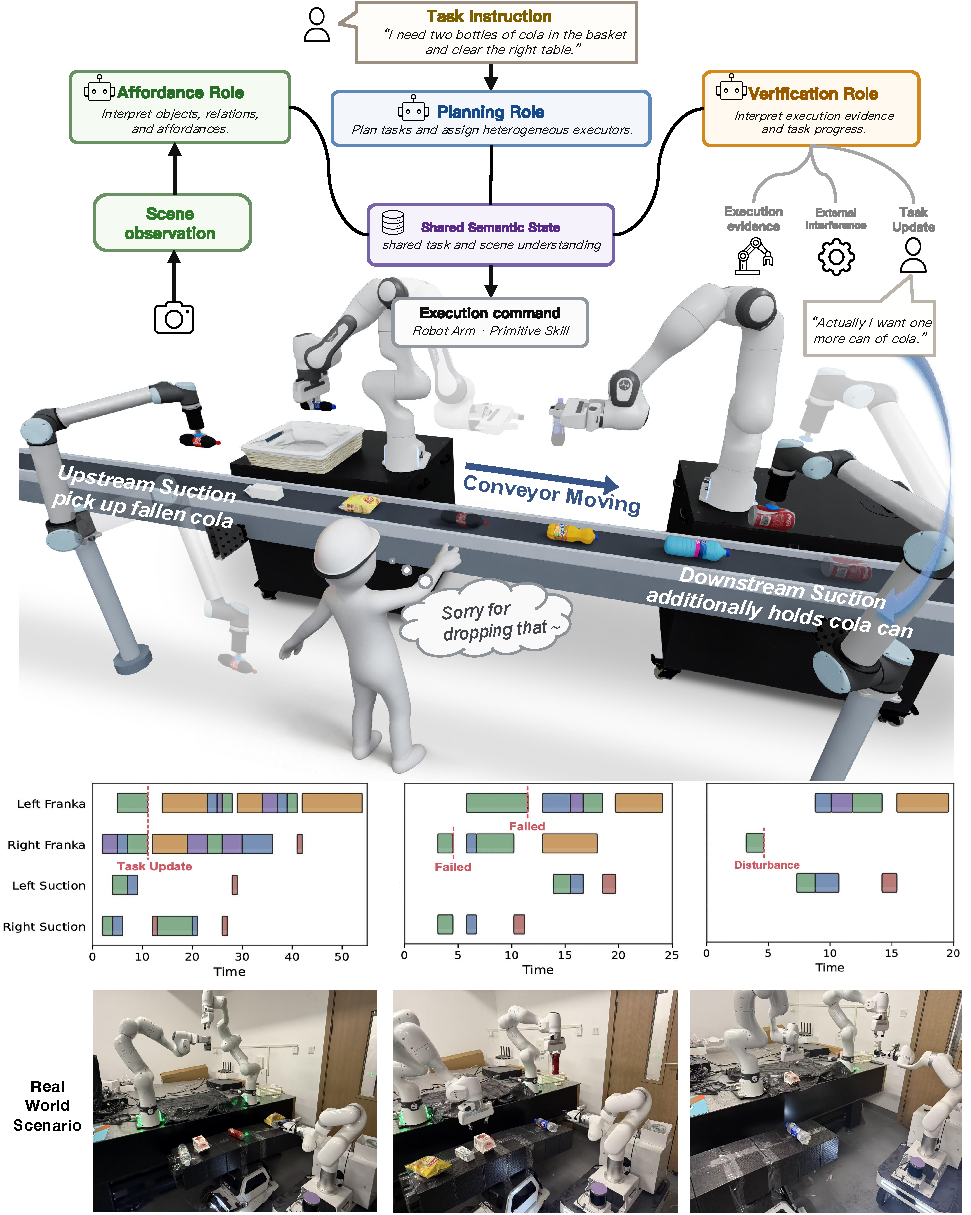
\includegraphics[width=\columnwidth]{figures/figure1_final_lowercase.pdf}
    \caption{The shared semantic state coordinates three roles while preserving
    local execution. \textbf{Top:} framework and simulated conveyor workspace;
    \textbf{Middle:} event Gantt charts; \textbf{Bottom left:} normal hardware
    execution; \textbf{Bottom middle:} hardware task update; \textbf{Bottom
    right:} hardware external disturbance.}
    \label{fig:scenario}
\end{figure}

\begin{figure*}[!t]
  \centering
  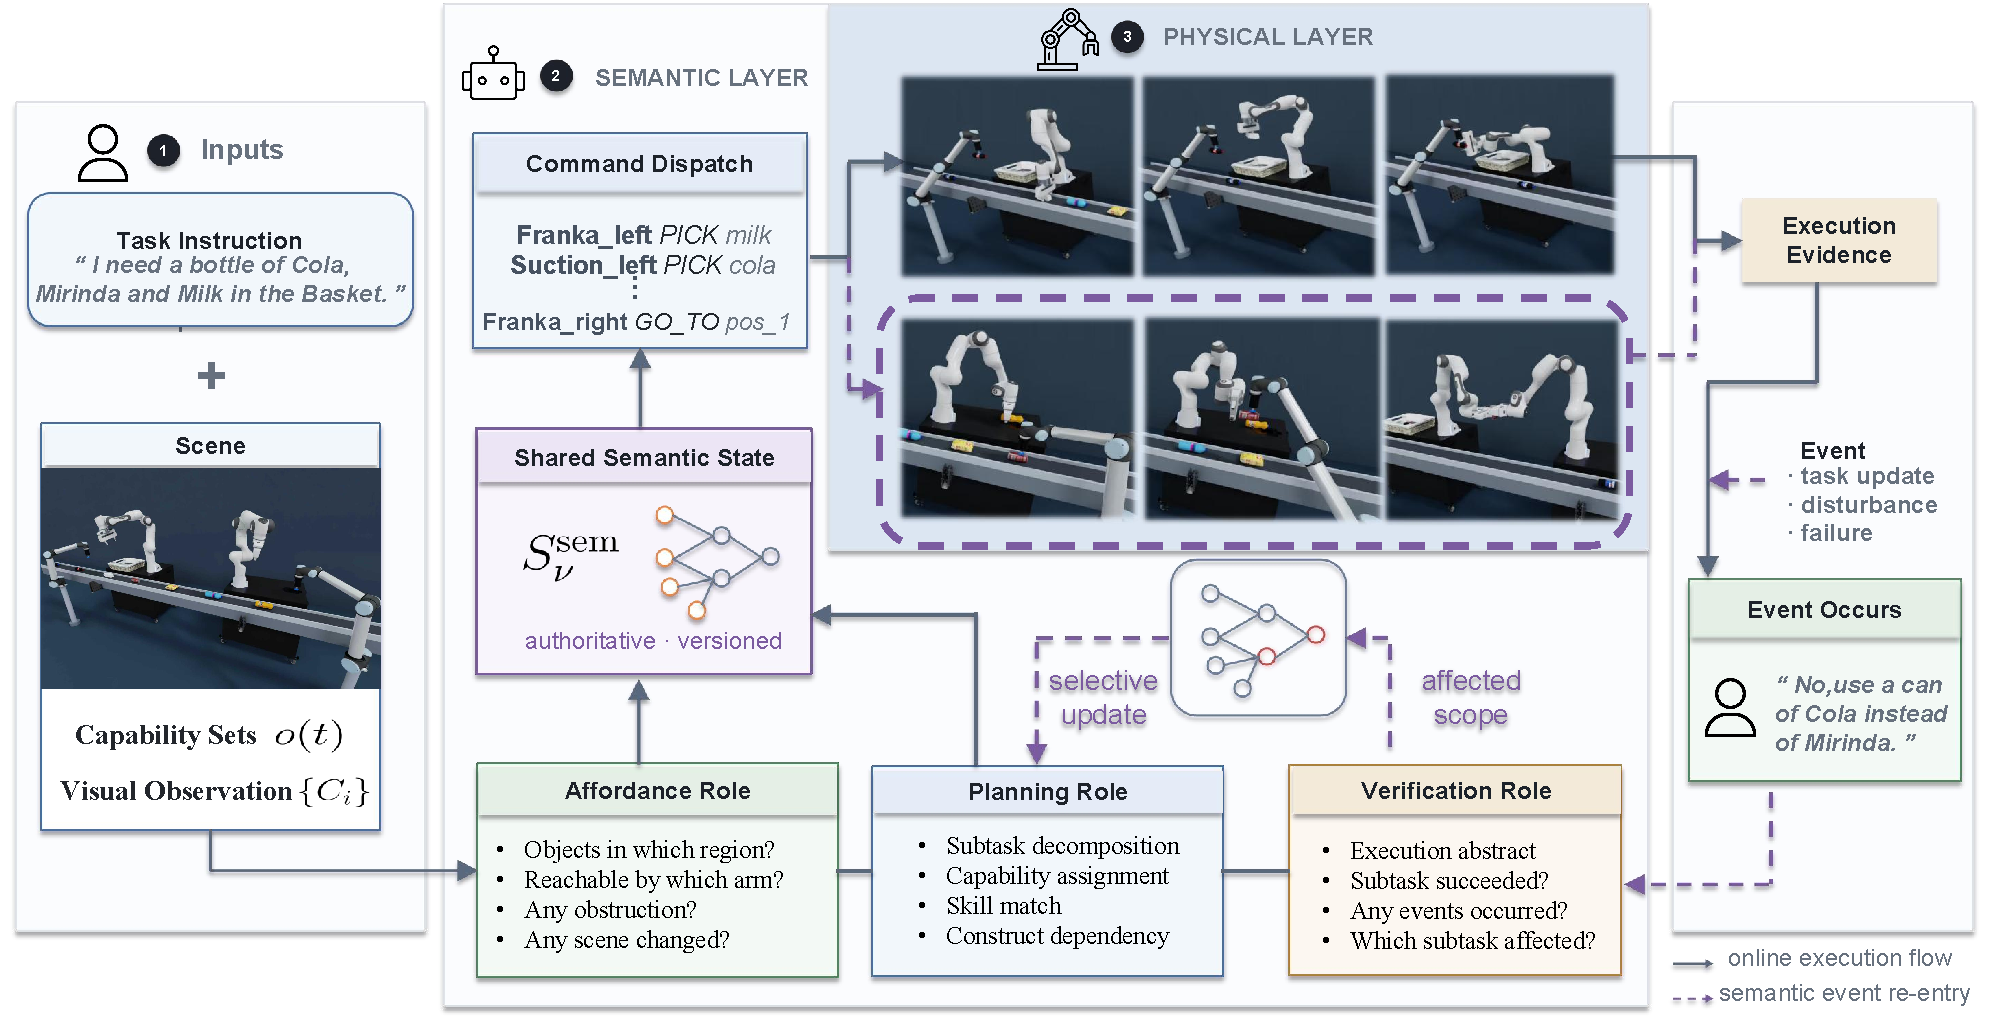
\includegraphics[width=0.96\textwidth]{figures/figure2.pdf}
  \caption{Role-shared coordination links semantic decisions to physical
  execution. Affordance evaluates scene feasibility; planning decomposes and
  assigns subtasks, skills, and dependencies; verification abstracts execution
  evidence, checks outcomes and events, and identifies affected subtasks. Solid
  and dashed arrows denote online execution and selective event updates.}
  \label{fig:method_overview}
\end{figure*}

\subsection{Related Work}
\label{sec:related_work}
\providecommand{\finalchange}[1]{#1}
\providecommand{\localexecchange}[1]{#1}

Language-guided grounding methods translate natural-language instructions into
spatial representations, executable programs, or scene-grounded task
plans~\cite{huang2023inner,liang2023code,rana2023sayplan,
huang2023voxposer}. Building on these capabilities, LLM-based multi-robot
frameworks adopt different coordination structures: RoCo uses inter-robot
dialogue; COHERENT relies on centralized proposals and execution feedback;
MALLVI reactivates specialized agents when needed; and CoMuRoS and DEXTER-LLM
revise tasks or assignments in response to events~\cite{
mandi2024roco,liu2025coherent,taji2026mallvi,
borate2026comuros,zhu2025dexter}. Other systems explicitly incorporate
capability-aware coalitions, dependency-based task allocation, or separate
planning, manipulation, and verification agents~\cite{
kannan2024smartllm,obata2025lipllm,he2026closedloop}. Collectively, these
methods establish effective mechanisms for grounding, agent interaction, and
task revision, but they do not explicitly organize ownership of the distinct
semantic components that must remain consistent as multiple heterogeneous
manipulators execute concurrently. RoSC addresses this issue by maintaining
the authoritative shared state and assigning responsibility
to the affordance, planning, and verification
roles, respectively. When a discrete semantic event occurs, these roles
identify its dependency-closed affected scope and reconstruct only the
invalidated subgraph, while preserving unaffected valid execution and leaving
continuous physical adaptation to the local controllers.


Dynamic manipulation supports tracked or reactive grasping and visual
servoing~\cite{marturi2019dynamic,maranci2026reactive,liu2023target,
haviland2020finalphase}, allowing local controllers to continuously adapt
end-effector motion to moving targets and perception updates. Execution
monitoring and continual replanning further address runtime deviations by
detecting discrepancies between expected and observed outcomes and invoking
recovery or plan revision~\cite{pettersson2005execution,brenner2009continual,
levihn2013foresight,pezzato2023active}. These methods primarily focus on
maintaining physical feasibility, monitoring action execution, or revising a
plan after deviations. However, in heterogeneous multi-manipulator settings,
the resulting feedback may affect different parts of the team-level semantic
state: a new observation may change an object's affordance, a failed action may
invalidate its execution status and downstream dependencies, and a revised
instruction may alter only one task branch. RoSC explicitly separates these
responsibilities among affordance, verification, and planning roles. It uses
the shared semantic state to determine which information must be refreshed,
which subtasks are affected, and whether planning should be invoked, thereby
supporting event-scoped semantic revision while preserving unaffected valid
execution.


\subsection{Our Method}
\label{sec:our_method_intro}

Figure~\ref{fig:method_overview} shows the resulting framework. At task start,
the affordance role evaluates object regions, reachability, obstructions, and
scene changes to produce $\mathcal{F}$; the planning role decomposes the task,
matches skills and capabilities to manipulators, constructs $G$, and initializes
the versioned shared semantic state
$S_\nu^{\texttt{sem}}=(\gamma,G,\mathcal{F},z)$. The framework then selects the
verified executable frontier, constructs capability-valid commands, and
dispatches independent commands concurrently to the assigned manipulators.
After local execution, affordance refreshes $\mathcal{F}$ and verification
abstracts the evidence, checks the outcome, updates $z$, and detects events. For
an event, verification identifies $\mathcal{N}_k^{\texttt{aff}}$; planning
replans that subgraph while preserving valid work outside it, then dispatch
continues from the updated frontier. This restricted semantic update shortens
the response path and helps preserve opportunities as the scene evolves.

The main contribution of this work is twofold: (I) A role-shared semantic
coordination formulation is introduced for dynamic heterogeneous
multi-manipulator scenarios with continual physical changes, assigning explicit
responsibility to the affordance, planning, and verification roles; and (II) An
event-driven selective semantic update procedure is developed to efficiently
handle task updates, external disturbances, and execution failures while
preserving unaffected valid execution.

%%========================================
\input{contents/problem.tex}
%%========================================
\input{contents/solution.tex}
%%========================================
\input{contents/experiment.tex}
%%========================================
\section{Conclusion}
\label{sec:conclusion}

This work proposes role-shared semantic coordination for dynamic heterogeneous
multi-arm manipulation with continual physical changes. The framework assigns
explicit semantic responsibilities to the affordance, planning, and
verification roles over a shared semantic state, and uses event-driven
selective updates to reconsider only the affected scope after task updates,
external disturbances, or execution failures. Within the tested heterogeneous
manipulation scenarios, baseline, ablation, and hardware results support role
separation for semantic responsibility allocation and selective updates for
efficient adaptation under semantic events.
The framework coordinates semantic decisions and semantic-state updates; it
does not replace local skill controllers, perception, low-level control, or
physical execution modules. The remaining execution boundary is visible in the
27/30 success rate for simulation execution failures and the 7/10 success rate
for the hardware disturbance condition, where physical uncertainty can still
prevent completion.

%%========================================

% \newpage
%========================================
\bibliographystyle{IEEEtran}
\bibliography{contents/references}



\end{document}
